\documentclass[tikz,border=3mm]{standalone}
\usepackage{amsmath}

\begin{document}

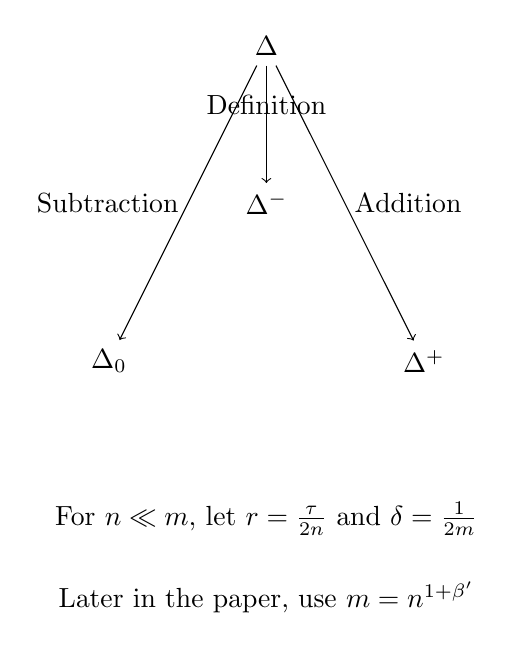
\begin{tikzpicture}[node distance=2cm]
    % Nodes
    \node (Delta) at (0,0) {\(\Delta\)};
    \node (DeltaMinus) at (0,-2) {\(\Delta^-\)};
    \node (DeltaZero) at (-2,-4) {\(\Delta_0\)};
    \node (DeltaPlus) at (2,-4) {\(\Delta^+\)};
    
    % Arrows and Labels
    \draw[->] (Delta) -- node[midway, above] {Definition} (DeltaMinus);
    \draw[->] (Delta) -- node[midway, left] {Subtraction} (DeltaZero);
    \draw[->] (Delta) -- node[midway, right] {Addition} (DeltaPlus);
    
    % Additional Information
    \node (info) at (0,-6) {For \(n \ll m\), let \(r = \frac{\tau}{2n}\) and \(\delta = \frac{1}{2m}\)};
    \node (example) at (0,-7) {Later in the paper, use \(m = n^{1 + \beta'}\)};
\end{tikzpicture}

\end{document}